\subsubsection{Electronic Devices and Nanophotonics}
\index{Knipp, Dietmar}

\paragraph{Electronic Devices and Nanophotonics group}
Dietmar Knipp (Professor), Amare Benor, Kah-Yoong Chan, Christian Haase (external PhD
student)  (PhD Student), Rahul Dewan (MSc student), Zhelio Andreev (MSc student)\\

Research of the Electronic Devices and Nanophotonics group is
focused on nano and optical technologies and their applications in
information technology and photovoltaics. The major goal of the
research is to develop the next generation of electronic and
photonic devices bridging from the micro to the nanoscale.

\paragraph{Highlights}

With the advent of micro and nano fabrication the production of nano-structured materials
in the sub 100 nm range became feasible. Such nanostructures are of interest for several
optical and photonic applications like solar cells and optical sensors.  For example, the
conversion efficiencies of thin film solar cells can be increased by nano texturing of the
cells. Due to nano texturing a larger fraction of the incoming light is scattered and
diffracted, so that the total absorption of light in the solar cell is
enhanced. Subsequently the generated photocurrent and the conversion efficiency of the
solar cell are enhanced. Despite these improvements the underlying optics in such nano
textured solar cells is not fully understood. Classical optics does not facilitate the
description of the wave propagation in such a solar cell. Maxwell's equations have to be
solved in 2D or 3D to gain insights in the optical wave propagation of such devices.  The
optics were studied by numerical simulations using a Finite Integration Technique (FIT)
and Finite Difference Time Domain (FDTD) approach. The device structure is approximated by
a solar cell with a periodic groove structure. The Figure~\ref{fig:profknipp1} (left)
shows one period of such a solar cell with a groove structure. The numerically simulated
absorption is shown in Figure~\ref{fig:profknipp1}, right.

\begin{figure}[ht]
  \begin{center}
    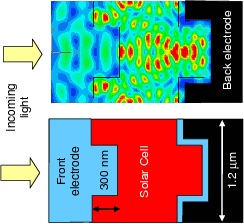
\includegraphics[width=\hsize, angle=270]{profknipp-figinfo.png}
    \mycaption{ Cross section of a slice of a nanotextured solar cell (left) and
      absorption profile in the solar cell}\label{fig:profknipp1}
   \end{center}
\end{figure}


The absorption of light in the cells is increased, due to scattering and diffraction of
light. Simulations carried out by Christian Haase show that the grooves cause an increase
of the total conversion efficiency of
10-15\%.
%The increase of the absorption is mainly observed for the infrared part of the
%optical spectrum. Based on a comparison of the experiment and the numerical
%simulation an optimized nano patterning schemes can be derived. The simulations show
%that the conversion efficiency is maximized if the height of the grooves is
%approximately equal to half of the period of the grooves.
The optical simulations were not only applied to solar cells. Numerical simulation of
metallic nanostructures shows that metallic hole arrays can be applied as optical
filters. The filter properties can be tuned by changing the diameter and the spacing of
the holes in the metal film. As the fabrication of the metallic structures is compatible
with classical micro and nanoelectronics such metallic nanostructures can be integrated in
conventional optical sensor or digital cameras. Cameras using such metallic nanostructures
would exhibit a reduced pixel cross talk and a higher spectral resolution.  In summary,
optics on the nanoscale provides a lot of new opportunities for technical
applications. Numerical simulations of the optics on the nanoscale are essential to gain a
solid understanding and optimize the device structures. In order to verify the results of
numerical simulations have to be compared to experimental results.  The research on
optics in nanostructured media is carried out in close collaboration with the research
group of Dr. H. Stiebig at the Institute of Photovoltaics, Research Center J\"ulich.

\paragraph{Collaborations}
\begin{enumerate}
\item {\sl International University Bremen} \\ Prof. Veit Wagner \\ Organic Electronics
\\ Prof. Werner Bergholz \\ Photovoltaics and Microelectronics
\item {\sl University Bremen} \\ Prof. Wolfgang Benecke \\ Microsystems Technology
\item {\sl Research Center J�lich} \\ Dr. Helmut Stiebig \\ Nanocrystalline Thin Film
  Transistors and Optics in nanostructured media
\item {\sl Bendit Innovative Interfaces} \\ J. Huyer \\ Solar Cells for mobile
  applications
\item {\sl Palo Alto Research Center} \\ Dr. R.A. Street, A.R. V�lkel. Dr. J. Northrup \\
  Organic electronics and modelling
\item {\sl Stanford University} \\ Prof. A. Salleo \\ Organic electronics

\end{enumerate}


\paragraph{Grants}
% list the running grants in 2006, if none have been received, please delete this
% subsection.
\begin{enumerate}
%\item {BMBF} ``Embedded Microsystems Bremen (EMB)''
\item Funded by {Forschungszentrum J\"ulich}, \emph{Funktionale
Kontaktschichen}, (February 2006 - January 2007)
\end{enumerate}


\paragraph{Awards, Prizes}
% list the grants you have received in 2005, if none have been received, please delete
% this subsection.
\begin{enumerate}
\item Ernst A.C. Lange Award together with Prof. W. Benecke from the Institute for
  Microsensors, -actuators, and -systems (University Bremen)
\end{enumerate}

\paragraph{Patents}
\begin{enumerate}
\item H. Stiebig, D. Knipp, J. F�lsch, Three-color sensor with a pin or nip series of
  layers, Japan, Patent number: Hei-9-535750;
\item D. Knipp, Optical sensor and integrated photonic crystal and method for producing
  the optical sensor, submitted to German patent office.
\end{enumerate}


\nocite{Knipp1, Knipp2, Knipp3, Knipp4, Knipp5, Knipp6, Knipp7, Knipp9,
Knipp10, Knipp11, Knipp13}
